\documentclass[11pt,a4paper]{article}

% ------------------------------------------------------------
% Encoding, language, and page layout
% ------------------------------------------------------------
\usepackage[T1]{fontenc}
\usepackage[utf8]{inputenc}
\usepackage[english]{babel}
\usepackage[a4paper,margin=2.5cm]{geometry}

% ------------------------------------------------------------
% Mathematics and units
% ------------------------------------------------------------
\usepackage{amsmath,amssymb}
\usepackage{siunitx}
\sisetup{
    detect-all,
    per-mode=symbol,
    output-decimal-marker={.}
}

% ------------------------------------------------------------
% Tables, figures, and links
% ------------------------------------------------------------
\usepackage{booktabs}
\usepackage{graphicx}
\usepackage{float}
\usepackage{caption}
\usepackage{hyperref}
\graphicspath{{figures/}}

\hypersetup{
    colorlinks=true,
    linkcolor=black,
    citecolor=black,
    urlcolor=blue
}

% ------------------------------------------------------------
% Document metadata
% ------------------------------------------------------------
\title{A Computational Geometric Approach to Center Distance Correction\\
       in Open Roller Chain Drives}
\author{Douglas Delorenzi Schons}
\date{\today}

\begin{document}

\maketitle

\begin{abstract}
This article presents a geometric formulation for calculating the corrected center distance in open roller chain drives. In a chain drive, the desired center distance between two sprockets does not necessarily correspond to a physically closable configuration, because the chain path is geometrically continuous while the real chain is composed of an integer number of links. The method calculates the sprocket pitch diameters, the continuous chain path length, the theoretical number of links, the selected integer link count, the actual chain length, and the corrected center distance. The corrected center distance is obtained by solving a nonlinear geometric closure equation after the link count has been discretized. A numerical example using an ASA 80 roller chain is presented and geometrically validated.
\end{abstract}

\noindent\textbf{Keywords:} roller chain drive; center distance correction; chain geometry; sprocket pitch diameter; link count discretization; mechanical design; Python engineering tool.

% ------------------------------------------------------------
\section{Introduction}
% ------------------------------------------------------------

Roller chain drives are widely used in mechanical power transmission systems due to their robustness, positive engagement, and relatively simple construction. However, even in a geometrically simple open chain drive with two sprockets, the desired center distance is not always directly compatible with the physical chain assembly.

The reason is that the theoretical chain path length is a continuous geometric quantity, while the real chain length is constrained by the chain pitch and by an integer number of links. Therefore, after selecting the nearest feasible link count, the original center distance generally needs to be corrected so that the final chain path length matches the actual chain length.

This article focuses on the geometric formulation of this problem and its computational implementation. The goal is not to perform a complete mechanical selection of the chain drive, but to solve the geometric closure problem associated with pitch circles, tangent segments, wrap arcs, link count discretization, and center distance correction.

% ------------------------------------------------------------
\section{Problem Statement}
% ------------------------------------------------------------

Given an open roller chain drive with two sprockets, the objective is to calculate the corrected center distance that closes the chain path exactly after the number of links has been selected.

The main input parameters are:

\begin{itemize}
    \item chain pitch, $p$;
    \item number of teeth of the smaller sprocket, $z_1$;
    \item number of teeth of the larger sprocket, $z_2$;
    \item desired center distance, $a_0$.
\end{itemize}

The main output quantities are:

\begin{itemize}
    \item pitch diameters of both sprockets;
    \item pitch radii of both sprockets;
    \item initial continuous chain path length;
    \item theoretical number of links;
    \item selected integer number of links;
    \item actual chain length;
    \item corrected center distance;
    \item center distance correction;
    \item tangency points for geometric plotting.
\end{itemize}

% ------------------------------------------------------------
\section{Scope and Assumptions}
% ------------------------------------------------------------

The model considers an open single-strand roller chain drive with two coplanar sprockets and parallel shafts. The chain path is represented by the trajectory of the roller centers, and each sprocket is represented by its pitch circle.

The following assumptions are adopted:

\begin{itemize}
    \item the chain is represented by the path of the roller centers;
    \item the sprockets are represented by their pitch circles;
    \item the drive is open, with two external tangent spans;
    \item both sprocket axes are parallel;
    \item the number of links must be an integer;
    \item the selected link count is obtained by rounding the theoretical link count to the nearest integer.
\end{itemize}

This version does not consider transmitted power, chain tension, service factor, wear, elongation, lubrication, fatigue, shock loading, efficiency, or load-based chain selection. The scope is restricted to the geometric closure of the chain path.

For roller chains, an even number of links is usually preferred because standard chain assembly alternates inner and outer links. An odd number of links may be physically assembled by using an offset link. Therefore, odd link counts are accepted in the mathematical model, but the need for an offset link must be reported as a technical observation.

% ------------------------------------------------------------
\section{Sprocket Pitch Diameter}
% ------------------------------------------------------------

For a roller chain with pitch $p$ and a sprocket with $z$ teeth, the sprocket pitch diameter is calculated by:

\begin{equation}
    D_p = \frac{p}{\sin\left(\frac{\pi}{z}\right)}
\end{equation}

where $D_p$ is the sprocket pitch diameter, $p$ is the chain pitch, and $z$ is the number of sprocket teeth.

For the smaller and larger sprockets:

\begin{equation}
    D_{p1} = \frac{p}{\sin\left(\frac{\pi}{z_1}\right)}
\end{equation}

\begin{equation}
    D_{p2} = \frac{p}{\sin\left(\frac{\pi}{z_2}\right)}
\end{equation}

The pitch radii are:

\begin{equation}
    r_1 = \frac{D_{p1}}{2}
\end{equation}

\begin{equation}
    r_2 = \frac{D_{p2}}{2}
\end{equation}

The radius difference is defined as:

\begin{equation}
    \Delta r = r_2 - r_1
\end{equation}

% ------------------------------------------------------------
\section{Open Chain Drive Geometry}
% ------------------------------------------------------------

Considering the desired center distance $a_0$, the sprocket centers are defined as:

\begin{equation}
    A = (0,0)
\end{equation}

\begin{equation}
    B = (a_0,0)
\end{equation}

The auxiliary tangent angle is given by:

\begin{equation}
    \sin(\phi_0) = \frac{\Delta r}{a_0}
\end{equation}

Therefore:

\begin{equation}
    \phi_0 = \arcsin\left(\frac{\Delta r}{a_0}\right)
\end{equation}

The length of each straight tangent span is:

\begin{equation}
    j_0 = \sqrt{a_0^2 - \Delta r^2}
\end{equation}

The wrap angles on the smaller and larger sprockets are:

\begin{equation}
    \alpha_{1,0} = \pi - 2\phi_0
\end{equation}

\begin{equation}
    \alpha_{2,0} = \pi + 2\phi_0
\end{equation}

The corresponding arc lengths are:

\begin{equation}
    L_{1,0} = r_1\alpha_{1,0}
\end{equation}

\begin{equation}
    L_{2,0} = r_2\alpha_{2,0}
\end{equation}

The initial continuous chain path length is:

\begin{equation}
    C_i = L_{1,0} + L_{2,0} + 2j_0
\end{equation}

or, equivalently:

\begin{equation}
    C_i(a_0) =
    \pi(r_1+r_2)
    +
    2\Delta r \arcsin\left(\frac{\Delta r}{a_0}\right)
    +
    2\sqrt{a_0^2 - \Delta r^2}
\end{equation}

\begin{figure}[H]
    \centering
    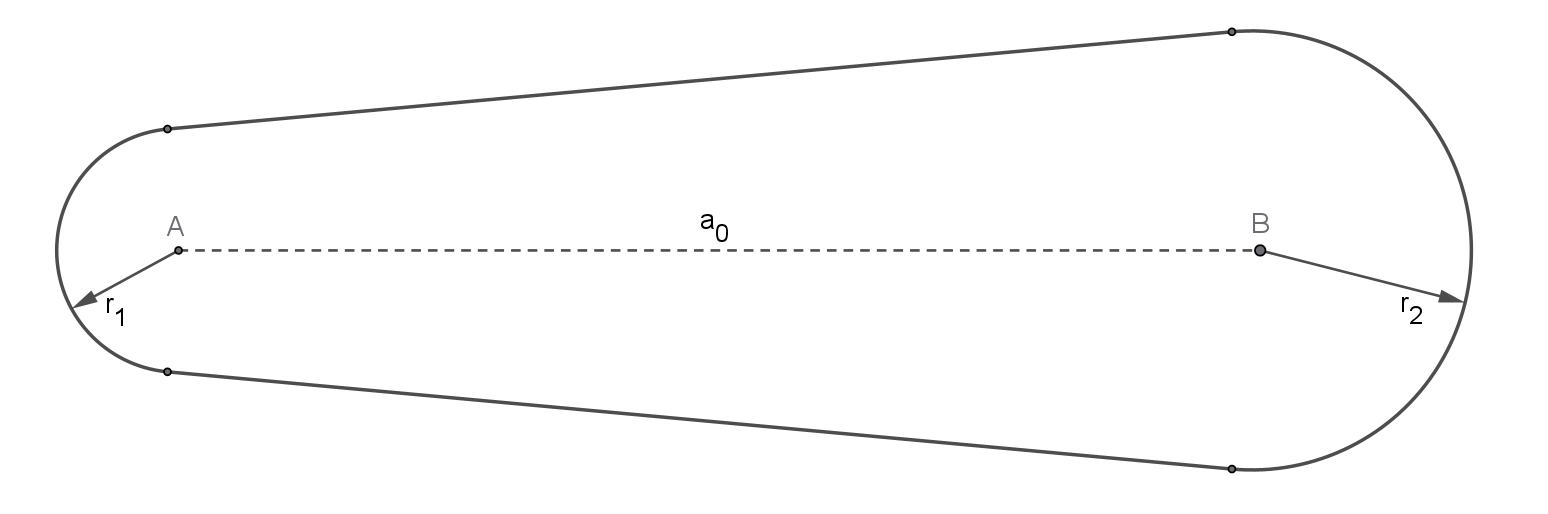
\includegraphics[width=0.95\textwidth]{figure_1.png}
    \caption{Geometric model of an open roller chain drive, showing the sprocket centers, pitch radii, center distance, tangent spans, and wrap arcs.}
    \label{fig:open-chain-geometry}
\end{figure}

% ------------------------------------------------------------
\section{Link Count Discretization}
% ------------------------------------------------------------

The theoretical number of links is obtained by dividing the initial continuous chain path length by the chain pitch:

\begin{equation}
    n_i = \frac{C_i}{p}
\end{equation}

The selected number of links is defined as the nearest integer:

\begin{equation}
    n = \operatorname{round}(n_i)
\end{equation}

The actual chain length is then:

\begin{equation}
    C = np
\end{equation}

The chain length mismatch before center distance correction is:

\begin{equation}
    e_C = C - C_i
\end{equation}

If $n$ is odd, the calculation remains mathematically valid, but the physical assembly requires an offset link.

\begin{figure}[H]
    \centering
    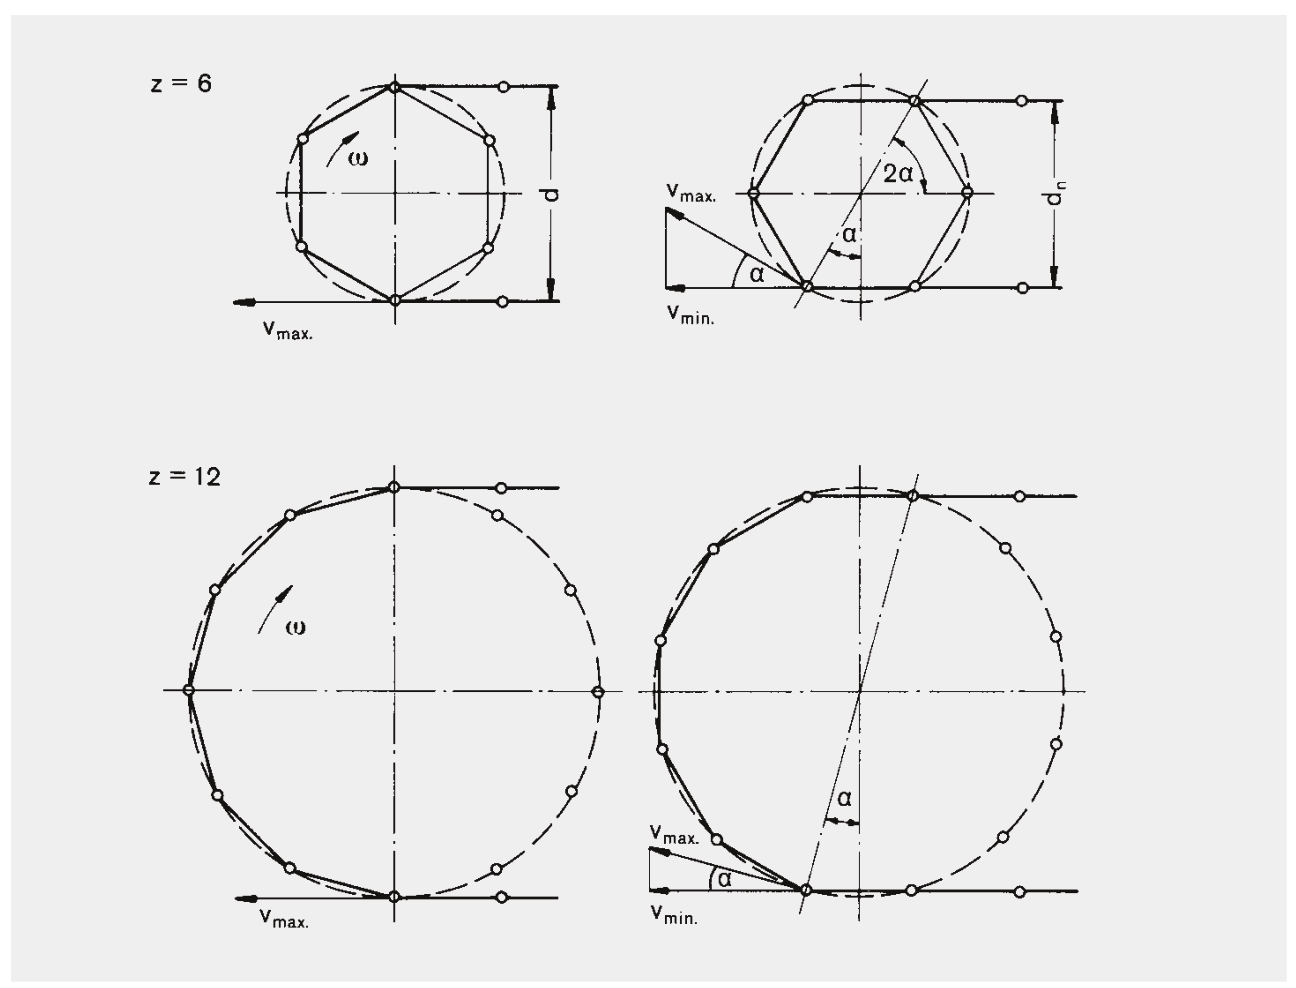
\includegraphics[width=0.85\textwidth]{figure_2.png}
    \caption{Pitch-based discretization in roller chain engagement. The pitch circle representation is a continuous geometric approximation, while the real chain is composed of discrete links and roller centers.}
    \label{fig:link-discretization}
\end{figure}

% ------------------------------------------------------------
\section{Corrected Center Distance}
% ------------------------------------------------------------

After the actual number of links has been selected, the corrected center distance $a_f$ must satisfy the geometric closure condition:

\begin{equation}
    C_i(a_f) = C
\end{equation}

where $C_i(a)$ is the continuous geometric chain path length and $C$ is the actual chain length after link count discretization.

The center distance function is physically meaningful only when the external tangent spans between the two sprocket pitch circles exist. Therefore, the center distance must satisfy:

\begin{equation}
    a > |\Delta r|
\end{equation}

where:

\begin{equation}
    \Delta r = r_2-r_1
\end{equation}

This condition also ensures that the square-root term remains real:

\begin{equation}
    \sqrt{a^2-\Delta r^2}
\end{equation}

Thus, the continuous chain path length function may be written as the following piecewise function:

\begin{equation}
    C_i(a) =
    \begin{cases}
    \pi(r_1+r_2)
    +
    2\Delta r \arcsin\left(\frac{\Delta r}{a}\right)
    +
    2\sqrt{a^2-\Delta r^2},
    & a > |\Delta r| \\[6pt]
    \text{undefined},
    & a \leq |\Delta r|
    \end{cases}
\end{equation}

The nonlinear error function is then defined as:

\begin{equation}
    f(a) = C_i(a) - C
\end{equation}

or explicitly, in the valid physical domain:

\begin{equation}
    f(a) =
    \pi(r_1+r_2)
    +
    2\Delta r \arcsin\left(\frac{\Delta r}{a}\right)
    +
    2\sqrt{a^2 - \Delta r^2}
    -
    C
\end{equation}

The corrected center distance is the root of this function:

\begin{equation}
    f(a_f) = 0
\end{equation}

which implies:

\begin{equation}
    C_i(a_f) = C
\end{equation}

The center distance correction is:

\begin{equation}
    \Delta a = a_f - a_0
\end{equation}

This is the central step of the formulation: the corrected center distance is obtained by solving a nonlinear geometric closure equation after the chain length has been discretized by the selected integer number of links.

\begin{figure}[H]
    \centering
    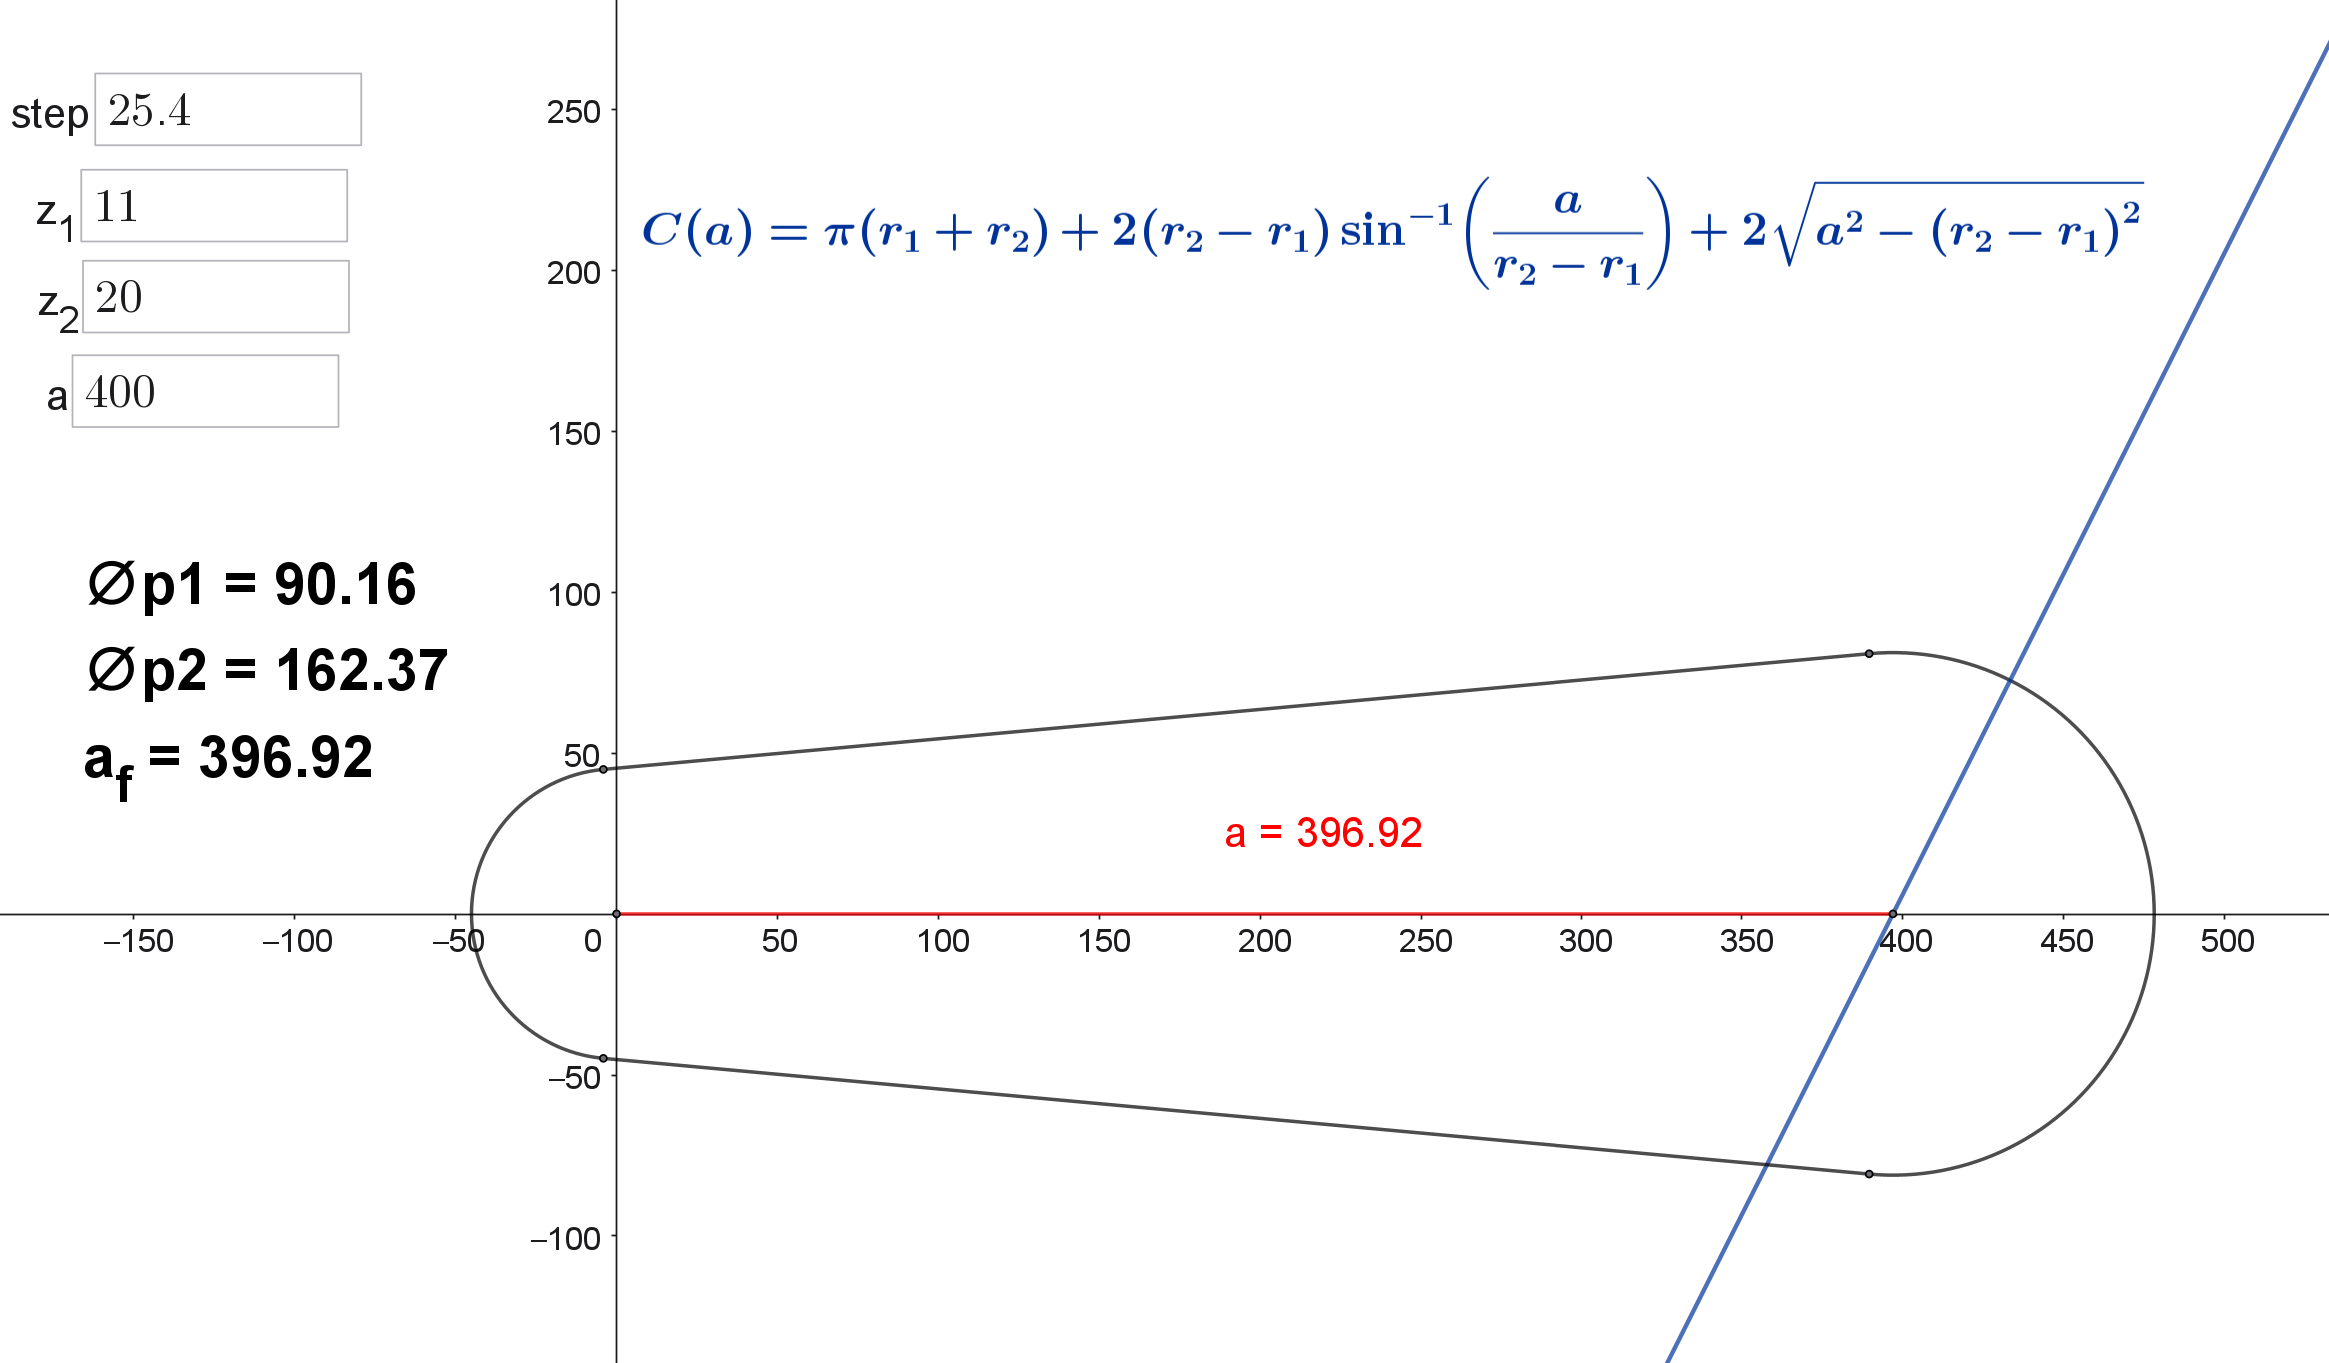
\includegraphics[width=0.95\textwidth]{figure_3.png}
    \caption{Error function used to determine the corrected center distance. The function is plotted only in the physically valid domain $a>|\Delta r|$, which ensures the existence of the external tangent spans and keeps the square-root term real. The corrected center distance is obtained at the root $f(a_f)=0$.}
    \label{fig:error-function}
\end{figure}

% ------------------------------------------------------------
\section{Tangency Points and Final Geometry}
% ------------------------------------------------------------

After determining the corrected center distance $a_f$, define:

\begin{equation}
    s_f = \frac{\Delta r}{a_f}
\end{equation}

\begin{equation}
    c_f = \frac{\sqrt{a_f^2 - \Delta r^2}}{a_f}
\end{equation}

The tangency points on the smaller sprocket pitch circle are:

\begin{equation}
    C_f = (-r_1s_f,\; r_1c_f)
\end{equation}

\begin{equation}
    D_f = (-r_1s_f,\; -r_1c_f)
\end{equation}

The tangency points on the larger sprocket pitch circle are:

\begin{equation}
    F_f = (a_f-r_2s_f,\; r_2c_f)
\end{equation}

\begin{equation}
    E_f = (a_f-r_2s_f,\; -r_2c_f)
\end{equation}

The final chain path is composed of:

\begin{itemize}
    \item the wrap arc on the smaller sprocket, from $C_f$ to $D_f$;
    \item the wrap arc on the larger sprocket, from $E_f$ to $F_f$;
    \item the upper tangent segment, from $C_f$ to $F_f$;
    \item the lower tangent segment, from $D_f$ to $E_f$.
\end{itemize}

% ------------------------------------------------------------
\section{Numerical Example}
% ------------------------------------------------------------

A chain drive using an ASA 80 roller chain is evaluated. The input data are:

\begin{itemize}
    \item chain pitch: $p = \SI{25.40}{mm}$;
    \item smaller sprocket: $z_1 = 11$ teeth;
    \item larger sprocket: $z_2 = 20$ teeth;
    \item desired center distance: $a_0 = \SI{400.00}{mm}$.
\end{itemize}

The calculated initial quantities are shown in Table~\ref{tab:initial-data}.

\begin{table}[H]
\centering
\caption{Initial data and pitch geometry for the ASA 80 example.}
\label{tab:initial-data}
\begin{tabular}{lr}
\toprule
Quantity & Value \\
\midrule
Chain pitch, $p$ & \SI{25.40}{mm} \\
Number of teeth, $z_1$ & 11 \\
Number of teeth, $z_2$ & 20 \\
Desired center distance, $a_0$ & \SI{400.00}{mm} \\
Smaller sprocket pitch diameter, $D_{p1}$ & \SI{90.16}{mm} \\
Larger sprocket pitch diameter, $D_{p2}$ & \SI{162.37}{mm} \\
Smaller sprocket pitch radius, $r_1$ & \SI{45.08}{mm} \\
Larger sprocket pitch radius, $r_2$ & \SI{81.18}{mm} \\
Radius difference, $\Delta r$ & \SI{36.11}{mm} \\
\bottomrule
\end{tabular}
\end{table}

For the desired center distance of \SI{400.00}{mm}, the initial continuous chain path length is:

\begin{equation}
    C_i = \SI{1199.93}{mm}
\end{equation}

The theoretical number of links is:

\begin{equation}
    n_i = 47.24
\end{equation}

Using nearest-integer rounding:

\begin{equation}
    n = 47
\end{equation}

Thus, the actual chain length is:

\begin{equation}
    C = 47 \cdot \SI{25.40}{mm} = \SI{1193.80}{mm}
\end{equation}

The initial length mismatch is:

\begin{equation}
    e_C = \SI{1193.80}{mm} - \SI{1199.93}{mm} = \SI{-6.13}{mm}
\end{equation}

Because the selected number of links is odd, the physical chain assembly requires an offset link.

Solving $f(a_f)=0$ gives:

\begin{equation}
    a_f = \SI{396.92}{mm}
\end{equation}

Therefore:

\begin{equation}
    \Delta a = \SI{396.92}{mm} - \SI{400.00}{mm} = \SI{-3.08}{mm}
\end{equation}

The center distance must be reduced from \SI{400.00}{mm} to approximately \SI{396.92}{mm} in order to close the selected 47-link chain.

% ------------------------------------------------------------
\section{Geometric Validation}
% ------------------------------------------------------------

The corrected geometry can be validated by summing the two wrap arcs and the two tangent segments:

\begin{equation}
    C_{\text{conf}} =
    L_{\text{small arc}}
    +
    L_{\text{large arc}}
    +
    L_{\text{upper tangent}}
    +
    L_{\text{lower tangent}}
\end{equation}

For the evaluated case:

\begin{equation}
    L_{\text{small arc}} = \SI{133.41}{mm}
\end{equation}

\begin{equation}
    L_{\text{large arc}} = \SI{269.84}{mm}
\end{equation}

\begin{equation}
    L_{\text{upper tangent}} = \SI{395.28}{mm}
\end{equation}

\begin{equation}
    L_{\text{lower tangent}} = \SI{395.28}{mm}
\end{equation}

Therefore:

\begin{equation}
    C_{\text{conf}} =
    \SI{133.41}{mm}
    +
    \SI{269.84}{mm}
    +
    \SI{395.28}{mm}
    +
    \SI{395.28}{mm}
    =
    \SI{1193.80}{mm}
\end{equation}

Since:

\begin{equation}
    C_{\text{conf}} = C
\end{equation}

the corrected geometry is considered validated for this numerical case.

\begin{figure}[H]
    \centering
    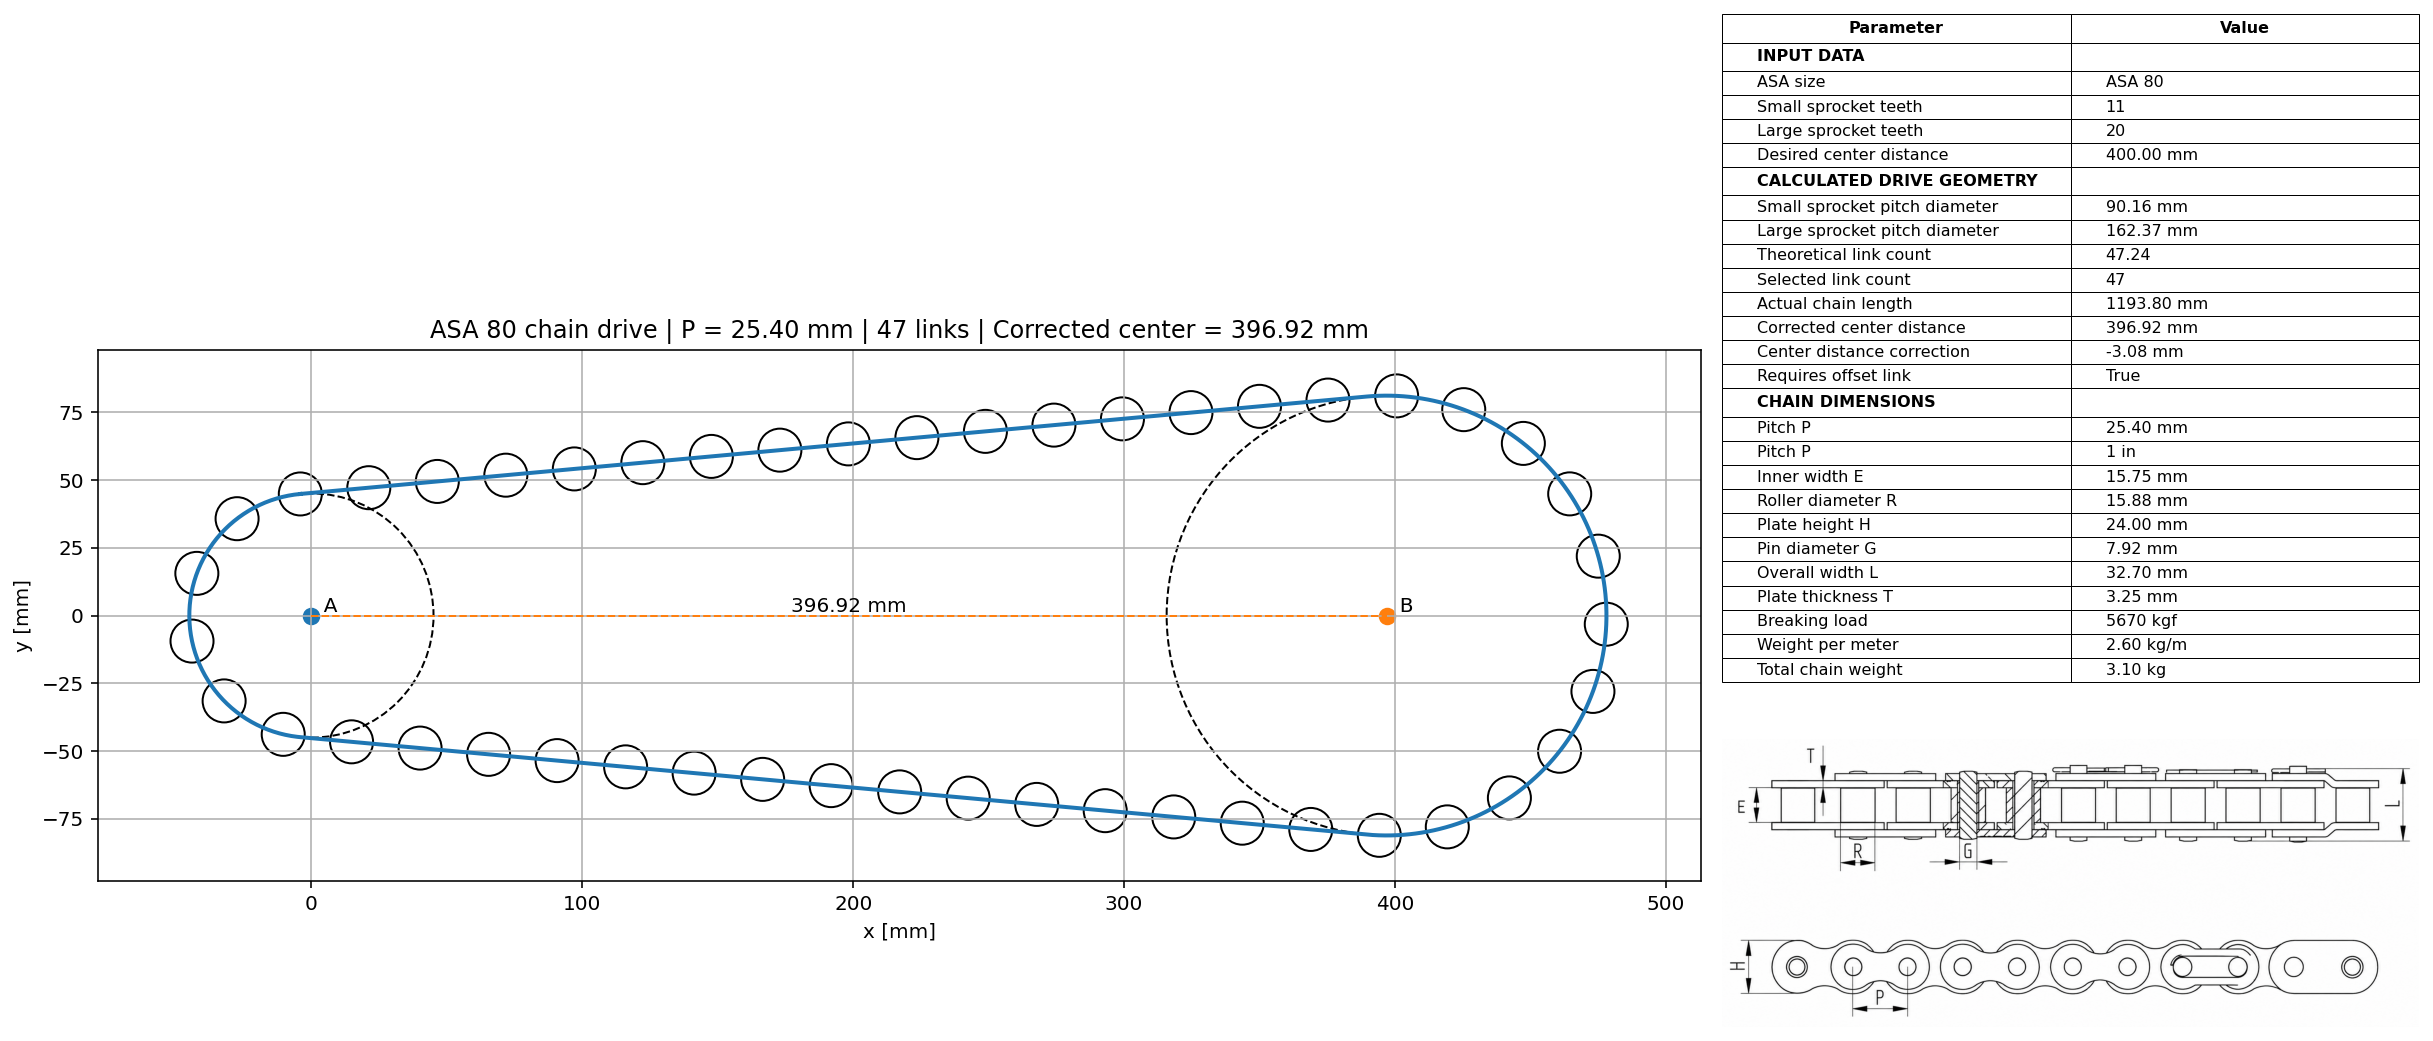
\includegraphics[width=1.00\textwidth]{figure_4.png}
    \caption{Computational output for the ASA 80 example, showing the corrected chain path, roller distribution, calculated parameters, and catalog chain dimensions.}
    \label{fig:corrected-geometry}
\end{figure}

% ------------------------------------------------------------
\section{Computational Implementation}
% ------------------------------------------------------------

The formulation was implemented as a Python-based engineering calculation tool. The main computational routine receives:

\begin{equation}
    (p,\; z_1,\; z_2,\; a_0)
\end{equation}

and returns:

\begin{itemize}
    \item sprocket pitch diameters;
    \item sprocket pitch radii;
    \item initial continuous chain path length;
    \item theoretical link count;
    \item selected integer link count;
    \item offset link requirement;
    \item actual chain length;
    \item corrected center distance;
    \item correction relative to the desired center distance;
    \item tangency points for plotting;
    \item chain mass estimate, when catalog weight data are available.
\end{itemize}

The same formulation can be used to generate plots, tables, technical reports, and interactive engineering tools.

% ------------------------------------------------------------
\section{Limitations and Future Work}
% ------------------------------------------------------------

The current formulation is restricted to geometric closure. It does not perform load-based chain selection or service life estimation.

Future work may include:

\begin{itemize}
    \item enforcing even link count as an optional design constraint;
    \item calculating chain speed;
    \item estimating transmitted power capacity;
    \item including service factors;
    \item evaluating chain tension;
    \item checking minimum sprocket tooth count recommendations;
    \item including lubrication and wear considerations;
    \item generating automatic PDF reports;
    \item creating a graphical or web-based interface.
\end{itemize}

% ------------------------------------------------------------
\section{Conclusion}
% ------------------------------------------------------------

The center distance correction problem in open roller chain drives illustrates how a classical mechanical design problem can be translated into a computational geometry workflow. The formulation combines pitch diameter calculation, open tangent geometry, wrap arc computation, link count discretization, and numerical solution of a nonlinear closure equation.

The key result is that the corrected center distance must be obtained after selecting the integer number of links, not before. In the evaluated ASA 80 example, a desired center distance of \SI{400.00}{mm} led to a theoretical link count of 47.24 links. After selecting 47 links, the corrected center distance became \SI{396.92}{mm}, requiring a reduction of \SI{3.08}{mm} from the initial design value.

This formulation is suitable for implementation in Python and can serve as the basis for an engineering software tool aimed at mechanical design, educational use, technical documentation, and portfolio demonstration.

\end{document}
